%-----------------------------------------------------
% Chapter 2: Características
%-----------------------------------------------------
\chapter{Marco teórico}
\label{chap: cap2}
\section{Desarrollo Colaborativo de Productos (CPD)}

La complejidad creciente de los productos, así como la personalización de los mismos a las particularidades de cada cliente, hace necesario la participación de especialistas para acortar los ciclos de desarrollo de producto y de puesta en el mercado. Tradicionalmente se consideraba la figura de contratistas, a los que se entregaban los planos para que construyeran las distintas partes que integran un proyecto de cualquier sistema. Los contactos se producían de forma presencial y obligaban a frecuentes viajes para mantener el proyecto bajo control. \vskip
En un esfuerzo por ahorrar tiempo y reducir los costos en las empresas, el Desarrollo Colaborativo de Productos del inglés \textit{Collaborative Product Development} (CPD) se ha expandido hace décadas.\vskip
El concepto teórico de CPD como lo conocemos hoy en día tuvo su primer aparición en 1994, en un artículo de Peter Cassidy \footnote{URL Google Book} en la revista CIO titulado "Multimedia Comes of Age". Sin embargo, la colaboración en el desarrollo de productos tiene antecedentes anteriores en el libro "The sources of innovation" de Eric Von Hippel \cite{VonHippel1988} en 1988. 
En 1995 apareció en más publicaciones como Complexities of Collaborative Product Development de MargaretBruce, Fiona Leverick y Dale Littler \cite{Complex1995}. En esa época el enfoque se hacía sobre la relación entre compradores y proveedores, la complejidad misma del desarrollo colaborativo de productos y sus factores de éxito. Posteriormente, la temática fué apareciendo con más frecuencia en artículos periodísticos y presentaciones de papers en todo el mundo. Obviamente esto no excluye la posibilidad de existencia de conceptos anteriores similares o equivalentes. 


\textbf{Algunas definiciones:}
En 1995, Bruce, Leverick y Littler \cite{Complex1995} describieron la visión de CPD como un medio efectivo para reducir el tiempo de desarrollo y el riesgo organizacional. Además declararon que el desarrollo colaborativo de productos es una proceso evolutivo y cómo la forma, el alcance de su iniciación y la continuación pueden cambiar en el tiempo.
El CPD está definido por la \textit{Product Development Management Association} \footnote{http://www.pdma.org/} desde 1996 como: "... cuando dos o más empresas deciden colaborar en el desarrollo de productos como socios mutuos, y esto difiere del concepto de externalización por el nivel de asociatividad, ya que las empresas colaboradoras están vinculadas en el proceso de entregar la solución final al cliente o al usuario." \vskip
Si bien con esta definición se puede comprender al CPD como colaboración entre agentes externos, hay otras como la de R. Del Rosario \cite{Mesbah2007} en el 2003 que lo describe como "la aplicación de prácticas de colaboración en equipo a los esfuerzos de desarrollo de productos dentro de una organización y además abarca la concurrencia, la atención al ciclo de vida, los proveedores y la tecnología de información en un entorno centrado en el cliente". 

Con respecto a la toma de desiciones, Marija Jankovic\cite{Marija2006} describe las implicaciones del contexto industrial colaborativo moderno durante el proceso de desarrollo del producto: \textit "En este proceso, cada actor tiene objetivos definidos para su dominio de acción. Por lo tanto, la toma de decisiones en colaboración es un proceso donde los actores tienen objetivos diferentes y a menudo contradictorios. Los actores en el proceso colaborativo de toma de decisiones tienen también diferentes grados de conocimientos sobre el problema, así como diferentes informaciones y puntos de vista." 

En este trabajo final el concepto de CPD no se usa específicamente para la colaboración externa o interna de una empresa, sino que incluye elementos de colaboración y toma de decisiones entre personas independientemente de la organización a la que pertenece, por ejemplo: la colaboración para diseñar un producto entre un diseñador industrial y una persona sin formación específica como puede ser un emprendedor.\vskip
En este contexto, el diseño tiene una importancia fundamental, ya que incorpora la información que define todos los pasos, hasta la elaboración final del producto. Puede decirse que la máxima eficacia se logra mediante la adecuación de esta etapa y es lo que realmente influye en el resultado final del producto.\vskip 

\textcolor{red}{
Para una efectiva colaboración no basta con una comunicación iterativa en la que se intercambian pocos datos del producto y siempre de arriba abajo (“top-down”), sino que es necesario disponer de un repositorio común de datos que vayan más allá de la geometría representada en planos, incluyendo documentos de especificaciones, instrucciones de
montaje, etc., y todos ellos en cualquier formato digital: texto, CAD/CAM/CAE, PDM, audio, vídeo y combinaciones de ellos.
Saber trabajar en colaboración se convierte en un valor agregado, sobre todo si ésta es suministradora de componentes o sistemas para ser integrados en el producto final y para lograr esto es indispensable aprovechar el contexto actual de las nuevas tecnologías web y sus posibilidades. \cite{Ruiz} }

\subsection{Diseño}
\say{ISO 9000:2000, la Norma que contiene el vocabulario de la Familia ISO 9000, define DISEÑO (Y DESARROLLO) como:
Conjunto de procesos que transforma los requisitos en características especificadas, o en la especificación de un producto, proceso, o sistema.\vskip
Perdiendo un poco de rigor, Diseñar es crear o definir cómo debe ser algo que satisface nuestros requisitos. Se trata de idear algo que no existe, o que no sabemos que existe. Sabemos qué función debe cumplir “ese algo”, pero no cómo debe ser, necesitamos diseñarlo.}  \footnote{http://www.portalcalidad.com/articulos/52-disenoproductosiso9001} Ver fig. 2.1

\begin{figure}
\centering
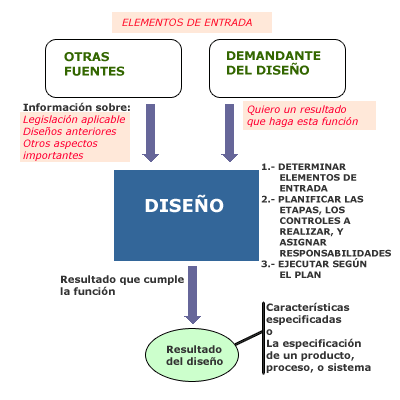
\includegraphics[width=12cm]{Img/CPD/0-CPD.png}
\caption[(optional short caption)]{\label{us_figure} Proceso de diseño de un producto – Patrón Conceptual}
\end{figure}



\subsection{Co-diseño}

La irrupción del diseño colaborativo como paradigma está cambiando el panorama de la práctica del diseño porque está permitiendo la aparición de nuevos dominios de creatividad colectiva. 

El co-diseño o diseño colaborativo se refiere a cómo se aplica la creatividad colectiva a través de toda la duración de un proceso de diseño. El concepto ha surgido tanto como un efecto de la globalización como también gracias a que se considera una potencial herramienta con la cual enfocar el desarrollo de productos, en una industria que requiere
nuevas tecnologías y procesos para abordar el diseño de artefactos cada vez más complejos y satisfacer de esta manera las altas expectativas de los clientes. 
El co-diseño es definido por el hecho de que la creatividad de los diseñadores se une a la de personas que tienen otros perfiles y trabajan juntas en el proceso de elaboración del diseño.
En esta definición se plantean los dos elementos fundamentales que soportan el
paradigma de diseño colaborativo:

\textbf{a) Nuevos perfiles}\vskip
En esta nueva forma de ver el diseño, al grupo habitual de trabajo se suman la iniciativa y la creatividad de otros perfiles que hasta ahora aportaban ideas generalmente como agentes externos: el investigador, el cliente y la persona que finalmente se beneficiará con el
resultado del co-diseño: el usuario.
En el diseño colaborativo estos perfiles tienden a mezclarse: El usuario pasa a jugar un rol de “experto en su experiencia” y puede aportar elementos de valor en la generación de conceptos e ideas en una etapa inicial de desarrollo. La labor del investigador, a partir de la experiencia del usuario, será proporcionar herramientas acertadas para recoger todos los datos que dicho perfil puede aportar y, a la vez, puede desempeñar un papel fundamental en dar forma a las ideas. De ahí la idea de que el investigador y el diseñador puede ser la misma persona.

\textbf{b) Objetivo en común}\vskip
La idea del objetivo compartido se plantea como una de las principales diferencias con respecto a los métodos tradicionales del diseño de productos o artefactos. Los métodos de diseño generalmente se planteaban para ser llevados a cabo por expertos que
realizaban tareas individuales. Con el trabajo individual no era necesario compartir la visión del objetivo general del proceso de diseño. En cambio, el diseño colaborativo plantea que este punto es fundamental: Para que el equipo funcione correctamente necesita tener la visión del objetivo en común.

Lógicamente, después de apuntar las características principales del diseño colaborativo, se infiere que el rol del diseñador en el proceso debe cambiar necesariamente al incluir este nuevos “socios” creativos en un entorno que tradicionalmente le pertenecía. \cite{Huerta2013}

\begin{figure}
\centering
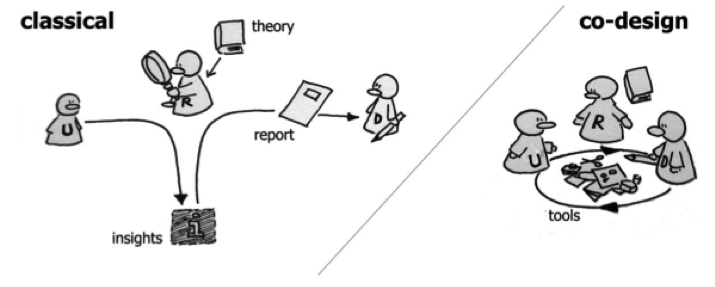
\includegraphics[width=12cm]{Img/CPD/1-CO.png}
\caption[(optional short caption)]{\label{us_figure} Diseño Clásico vs Co-diseño}
\end{figure}

\textcolor{red}{Desarrollar la parte de CAD parametrico y la relacion con CPD}

\begin{figure}
\centering
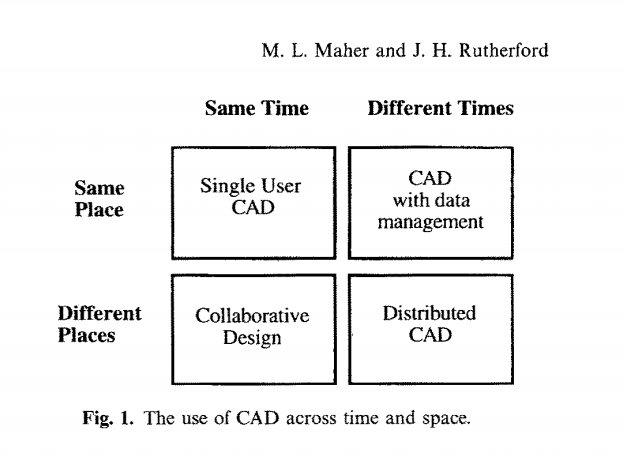
\includegraphics[width=12cm]{Img/CPD/2-CAD.png}
\caption[(optional short caption)]{\label{us_figure} El uso del CAD a través del tiempo y espacio}
\end{figure}


\subsection{Diseño paramétrico}

El \textbf{Diseño Paramétrico} se entiende en términos generales como un proceso de descripción de una problemática utilizando variables. Para describir estas variables, los diseñadores
insertan valores numéricos o algoritmos en un software especializado, y al cambiar las
variables se generan una serie de alternativas de soluciones, y según el criterio del diseñador, la solución final es creada. Davis (2013) y Hudson (2010) concuerdan en que el diseño paramétrico en su definición contemporánea es únicamente posible creando un \textbf{modelo paramétrico}. Esto lo definen como un conjunto de ecuaciones que expresan una geometría explícitamente por medio de funciones definidas por parámetros. Esta representación se basa en las relaciones entre estas variables. Todo sistema de esta índole está compuesto por unos parámetros iniciales y las relaciones entre ellos, de manera que si se ajusta uno de los parámetros, el resultado se verá afectado de manera acorde, al igual que si se altera alguna de las relaciones. Esto brinda una característica de fuerte y sencilla maleabilidad, que permite verificar resultados fácilmente. El diseñador que emplea estas herramientas en vez de diseñar un objeto resultante, se enfoca en crear lógicas que pongan en relación estos parámetros y resulten en un sistema vivo y ampliamente modificable de acuerdo al criterio del diseñador, asistido por la
computadora. El uso de este método por medio de la manipulación de los sistemas fomenta la exploración y la experimentación de las formas del producto, que se generan automáticamente por la modificación de los parámetros o las relaciones. Woodbury (2010) afirma que el diseño es cambio y que el modelado paramétrico representa el cambio. Esto lo menciona como una característica esencial del diseño paramétrico, como aquello que lo distingue de los métodos de diseño tradicionales. Es marcar e identificar
las partes y como se relacionan y cambian de manera coordinada. (Woodbury, 2010). La demostración explicita de las partes es lo que contribuye a la intervención y modificación
interactiva en tiempo real, debido a la operatividad visible del cambio en el sistema. La
lógica sistemática del diseño paramétrico permite evaluar las relaciones de manera visible, en lugar de hacerlo de manera intuitiva por medio de un proceso mental interno.
Esto le permite al diseñador explorar y descubrir nuevas posibilidades en lugar de hurgar
en sus conocimientos previos para llegar con una solución que ya conocía (Cross, 2006).
Este autor también afirma que es necesaria una representación visual ya que diseñar es difícil de conducir puramente por procesos mentales internos (Cross, 2011, p. 12).\vskip
\textcolor{red}{

En este trabajo se optó por la utilización de modelos 3D paramétricos porque para lograr la colaboración es indispensable que los diseños se generen en función de sus parámetros y además expongan sus características de manera comprensible por todas las partes involucradas. Por ejemplo: un diseñador industrial puede comprender naturalmente parámetros como arista, vértices o normales pero un artista puede comprender sobre dimensiones, colores o materiales. Por ende es recomendable que los modelos 3D en este caso se expongan en función de los parámetros conocidos por el artista.}
\textcolor{red}{Para ello surge la necesidad de mecanismos de manipulación directa de los modelos 3D por parte de los interesados para posibilitar la generación de nuevas versiones o soluciones, y así gracias al diseño iterativo lograr la colaboración.} 


\begin{figure}
\centering
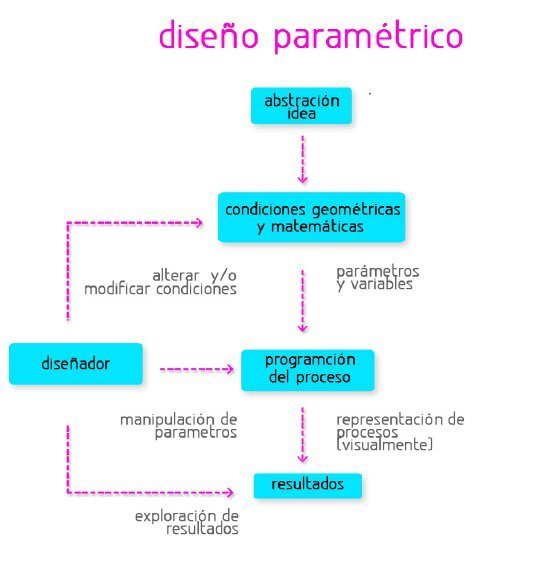
\includegraphics[width=12cm]{Img/CPD/4-PARAM.jpg}
\caption[(optional short caption)]{\label{us_figure} Proceso de diseño paramétrico }
\end{figure}


\subsection{CAD especificado en algoritmos} 
El diseño asistido por ordenador (CAD – Computer Aided Design), se utiliza para generar modelos con las principales características de un determinado producto, manipulando con gran facilidad los datos geométricos. 

http://www.patrikschumacher.com/Texts/Design%20Parameters%20to%20Parametric%20Design.html

Las herramientas de diseño asistido por computadora CAD tradicionales fueron pensadas para un usuario, por ende tienen limitaciones para soportar el entorno de desarrollo colaborativo de productos y de forma rápida como requiere el mercado. Actualmente el desarrollo de productos es el resultado de procesos colaborativos basados en la red, porque la mayoría de los proyectos requieren la cooperación entre actores distribuidos geográficamente. En un proceso de desarrollo distribuido, se necesita una comunicación efectiva y de alta velocidad. La mayoría de los errores de diseño se deben a la falta de comunicación entre los equipos de diseño distribuidos.
Los sistemas de información distribuída que se han aplicado para CPD se pueden clasificar en 3: web services, remote services y remote repositories.Los sistemas basados en web services tienen ventajas sobre los otros dos porque son relativamente sencillos de diseñar e implementar, reducen los problemas de la instalación de software y facilita la posibilidad de la colaboración. \cite{Nyamsuren2015}



Articulo: Collaborative 3D Workspace and Interaction Techniques
for Synchronous Distributed Product Design Reviews. 
Emergence in collaborative computer-aided design


\subsection{Visualización de modelos 3D. Data exchange
}

\subsection{Sistemas de persistencia y parámetros
}

\subsection{Interfaces de manipulación directa}

\section{Trabajos relacionados y antecedentes}

\section{Problemas y recomendaciones
}